% !Mode:: "TeX:UTF-8"
\documentclass{article}

%%%%%%%%------------------------------------------------------------------------
%%%% 日常所用宏包

%% 控制页边距
% 如果是beamer文档类, 则不用geometry
\makeatletter
\@ifclassloaded{beamer}{}{\usepackage[top=2.5cm, bottom=2.5cm, left=2.5cm, right=2.5cm]{geometry}}
\makeatother

%% 控制项目列表
\usepackage{enumerate}

%% 多栏显示
\usepackage{multicol}

%% 算法环境
\usepackage{algorithm}  
\usepackage{algorithmic} 
\usepackage{float} 

%% 网址引用
\usepackage{url}

%% 控制矩阵行距
\renewcommand\arraystretch{1.4}

%% hyperref宏包,生成可定位点击的超链接,并且会生成pdf书签
\makeatletter
\@ifclassloaded{beamer}{
\usepackage{hyperref}
}{
\usepackage[%
    pdfstartview=FitH,%
    CJKbookmarks=true,%
    bookmarks=true,%
    bookmarksnumbered=true,%
    bookmarksopen=true,%
    colorlinks=true,%
    citecolor=blue,%
    linkcolor=blue,%
    anchorcolor=green,%
    urlcolor=blue%
]{hyperref}
}
\makeatother



\makeatletter % 如果是 beamer 不需要下面两个包
\@ifclassloaded{beamer}{

}{
%% 控制标题
\usepackage{titlesec}
%% 控制目录
\usepackage{titletoc}
}
\makeatother

%% 控制表格样式
\usepackage{booktabs}

%% 控制字体大小
\usepackage{type1cm}

%% 首行缩进,用\noindent取消某段缩进
\usepackage{indentfirst}

%% 支持彩色文本、底色、文本框等
\usepackage{color,xcolor}

%% AMS LaTeX宏包: http://zzg34b.w3.c361.com/package/maths.htm#amssymb
\usepackage{amsmath,amssymb}

%%%% 基本插图方法
%% 图形宏包
\usepackage{graphicx}

%% 多个图形并排
\usepackage{subfig}

%%%% 基本插图方法结束

%%%% pgf/tikz绘图宏包设置
\usepackage{pgf,tikz}
\usetikzlibrary{shapes,automata,snakes,backgrounds,arrows}
\usetikzlibrary{mindmap}
%% 可以直接在latex文档中使用graphviz/dot语言,
%% 也可以用dot2tex工具将dot文件转换成tex文件再include进来
%% \usepackage[shell,pgf,outputdir={docgraphs/}]{dot2texi}
%%%% pgf/tikz设置结束


\makeatletter % 如果是 beamer 不需要下面两个包
\@ifclassloaded{beamer}{

}{
%%%% fancyhdr设置页眉页脚
%% 页眉页脚宏包
\usepackage{fancyhdr}
%% 页眉页脚风格
\pagestyle{plain}
}

%% 有时会出现\headheight too small的warning
\setlength{\headheight}{15pt}

%% 清空当前页眉页脚的默认设置
%\fancyhf{}
%%%% fancyhdr设置结束


\makeatletter % 对 beamer 要重新设置
\@ifclassloaded{beamer}{

}{
%%%% 设置listings宏包用来粘贴源代码
%% 方便粘贴源代码,部分代码高亮功能
\usepackage{listings}

%% 设置listings宏包的一些全局样式
%% 参考http://hi.baidu.com/shawpinlee/blog/item/9ec431cbae28e41cbe09e6e4.html
\lstset{
showstringspaces=false,              %% 设定是否显示代码之间的空格符号
numbers=left,                        %% 在左边显示行号
numberstyle=\tiny,                   %% 设定行号字体的大小
basicstyle=\footnotesize,                    %% 设定字体大小\tiny, \small, \Large等等
keywordstyle=\color{blue!70}, commentstyle=\color{red!50!green!50!blue!50},
                                     %% 关键字高亮
frame=shadowbox,                     %% 给代码加框
rulesepcolor=\color{red!20!green!20!blue!20},
escapechar=`,                        %% 中文逃逸字符,用于中英混排
xleftmargin=2em,xrightmargin=2em, aboveskip=1em,
breaklines,                          %% 这条命令可以让LaTeX自动将长的代码行换行排版
extendedchars=false                  %% 这一条命令可以解决代码跨页时,章节标题,页眉等汉字不显示的问题
}}
\makeatother
%%%% listings宏包设置结束


%%%% 附录设置
\makeatletter % 对 beamer 要重新设置
\@ifclassloaded{beamer}{

}{
\usepackage[title,titletoc,header]{appendix}
}
\makeatother
%%%% 附录设置结束


%%%% 日常宏包设置结束
%%%%%%%%------------------------------------------------------------------------


%%%%%%%%------------------------------------------------------------------------
%%%% 英文字体设置结束
%% 这里可以加入自己的英文字体设置
%%%%%%%%------------------------------------------------------------------------

%%%%%%%%------------------------------------------------------------------------
%%%% 设置常用字体字号,与MS Word相对应

%% 一号, 1.4倍行距
\newcommand{\yihao}{\fontsize{26pt}{36pt}\selectfont}
%% 二号, 1.25倍行距
\newcommand{\erhao}{\fontsize{22pt}{28pt}\selectfont}
%% 小二, 单倍行距
\newcommand{\xiaoer}{\fontsize{18pt}{18pt}\selectfont}
%% 三号, 1.5倍行距
\newcommand{\sanhao}{\fontsize{16pt}{24pt}\selectfont}
%% 小三, 1.5倍行距
\newcommand{\xiaosan}{\fontsize{15pt}{22pt}\selectfont}
%% 四号, 1.5倍行距
\newcommand{\sihao}{\fontsize{14pt}{21pt}\selectfont}
%% 半四, 1.5倍行距
\newcommand{\bansi}{\fontsize{13pt}{19.5pt}\selectfont}
%% 小四, 1.5倍行距
\newcommand{\xiaosi}{\fontsize{12pt}{18pt}\selectfont}
%% 大五, 单倍行距
\newcommand{\dawu}{\fontsize{11pt}{11pt}\selectfont}
%% 五号, 单倍行距
\newcommand{\wuhao}{\fontsize{10.5pt}{10.5pt}\selectfont}
%%%%%%%%------------------------------------------------------------------------


%% 设定段间距
\setlength{\parskip}{0.5\baselineskip}

%% 设定行距
\linespread{1}


%% 设定正文字体大小
% \renewcommand{\normalsize}{\sihao}

%制作水印
\RequirePackage{draftcopy}
\draftcopyName{XTUMESH}{100}
\draftcopySetGrey{0.90}
\draftcopyPageTransform{40 rotate}
\draftcopyPageX{350}
\draftcopyPageY{80}

%%%% 个性设置结束
%%%%%%%%------------------------------------------------------------------------


%%%%%%%%------------------------------------------------------------------------
%%%% bibtex设置

%% 设定参考文献显示风格
% 下面是几种常见的样式
% * plain: 按字母的顺序排列,比较次序为作者、年度和标题
% * unsrt: 样式同plain,只是按照引用的先后排序
% * alpha: 用作者名首字母+年份后两位作标号,以字母顺序排序
% * abbrv: 类似plain,将月份全拼改为缩写,更显紧凑
% * apalike: 美国心理学学会期刊样式, 引用样式 [Tailper and Zang, 2006]

\makeatletter
\@ifclassloaded{beamer}{
\bibliographystyle{apalike}
}{
\bibliographystyle{unsrt}
}
\makeatother


%%%% bibtex设置结束
%%%%%%%%------------------------------------------------------------------------

%%%%%%%%------------------------------------------------------------------------
%%%% xeCJK相关宏包

\usepackage{xltxtra,fontspec,xunicode}
\usepackage[slantfont, boldfont]{xeCJK} 

%% 针对中文进行断行
\XeTeXlinebreaklocale "zh"             

%% 给予TeX断行一定自由度
\XeTeXlinebreakskip = 0pt plus 1pt minus 0.1pt

%%%% xeCJK设置结束                                       
%%%%%%%%------------------------------------------------------------------------

%%%%%%%%------------------------------------------------------------------------
%%%% xeCJK字体设置

%% 设置中文标点样式,支持quanjiao、banjiao、kaiming等多种方式
\punctstyle{kaiming}                                        
                                                     
%% 设置缺省中文字体
\setCJKmainfont[BoldFont={Adobe Heiti Std}, ItalicFont={Adobe Kaiti Std}]{Adobe Song Std}   
%% 设置中文无衬线字体
\setCJKsansfont[BoldFont={Adobe Heiti Std}]{Adobe Kaiti Std}  
%% 设置等宽字体
\setCJKmonofont{Adobe Heiti Std}                            

%% 英文衬线字体
\setmainfont{DejaVu Serif}                                  
%% 英文等宽字体
\setmonofont{DejaVu Sans Mono}                              
%% 英文无衬线字体
\setsansfont{DejaVu Sans}                                   

%% 定义新字体
\setCJKfamilyfont{song}{Adobe Song Std}                     
\setCJKfamilyfont{kai}{Adobe Kaiti Std}
\setCJKfamilyfont{hei}{Adobe Heiti Std}
\setCJKfamilyfont{fangsong}{Adobe Fangsong Std}
\setCJKfamilyfont{lisu}{LiSu}
\setCJKfamilyfont{youyuan}{YouYuan}

%% 自定义宋体
\newcommand{\song}{\CJKfamily{song}}                       
%% 自定义楷体
\newcommand{\kai}{\CJKfamily{kai}}                         
%% 自定义黑体
\newcommand{\hei}{\CJKfamily{hei}}                         
%% 自定义仿宋体
\newcommand{\fangsong}{\CJKfamily{fangsong}}               
%% 自定义隶书
\newcommand{\lisu}{\CJKfamily{lisu}}                       
%% 自定义幼圆
\newcommand{\youyuan}{\CJKfamily{youyuan}}                 

%%%% xeCJK字体设置结束
%%%%%%%%------------------------------------------------------------------------

%%%%%%%%------------------------------------------------------------------------
%%%% 一些关于中文文档的重定义
\newcommand{\chntoday}{\number\year\,年\,\number\month\,月\,\number\day\,日}
%% 数学公式定理的重定义

%% 中文破折号,据说来自清华模板
\newcommand{\pozhehao}{\kern0.3ex\rule[0.8ex]{2em}{0.1ex}\kern0.3ex}

\newtheorem{example}{例}                                   
\newtheorem{theorem}{定理}[section]                         
\newtheorem{definition}{定义}
\newtheorem{axiom}{公理}
\newtheorem{property}{性质}
\newtheorem{proposition}{命题}
\newtheorem{lemma}{引理}
\newtheorem{corollary}{推论}
\newtheorem{remark}{注解}
\newtheorem{condition}{条件}
\newtheorem{conclusion}{结论}
\newtheorem{assumption}{假设}

\makeatletter %
\@ifclassloaded{beamer}{

}{
%% 章节等名称重定义
\renewcommand{\contentsname}{目录}     
\renewcommand{\indexname}{索引}
\renewcommand{\listfigurename}{插图目录}
\renewcommand{\listtablename}{表格目录}
\renewcommand{\appendixname}{附录}
\renewcommand{\appendixpagename}{附录}
\renewcommand{\appendixtocname}{附录}
%% 设置chapter、section与subsection的格式
\titleformat{\chapter}{\centering\huge}{第\thechapter{}章}{1em}{\textbf}
\titleformat{\section}{\centering\sihao}{\thesection}{1em}{\textbf}
\titleformat{\subsection}{\xiaosi}{\thesubsection}{1em}{\textbf}
\titleformat{\subsubsection}{\xiaosi}{\thesubsubsection}{1em}{\textbf}

\@ifclassloaded{book}{

}{
\renewcommand{\abstractname}{摘要}
}
}
\makeatother

\renewcommand{\figurename}{图}
\renewcommand{\tablename}{表}

\makeatletter
\@ifclassloaded{book}{
\renewcommand{\bibname}{参考文献}
}{
\renewcommand{\refname}{参考文献} 
}
\makeatother

\floatname{algorithm}{算法}
\renewcommand{\algorithmicrequire}{\textbf{输入:}}
\renewcommand{\algorithmicensure}{\textbf{输出:}}

%%%% 中文重定义结束
%%%%%%%%------------------------------------------------------------------------

\setCJKmainfont{STKaiti} % 如果请替换为本地系统有的字体
%中文断行
\XeTeXlinebreaklocale "zh"
\XeTeXlinebreakskip = 0pt plus 1pt minus 0.1pt
\begin{document}
\title{}
%\date{\today}
\maketitle
%\tableofcontents
%\newpage
\section{连续高斯链模型}
连续高斯链是一种用于分析和数值计算的理想链模型,该模型可以被描述为离散高斯链模型的连续极限,其中的聚合物被视为一个连续的线性弹性丝。如图1所示,连续高斯链的构型由空间曲线$\mathbf{r}(s)$描述,其中$s\in [0,N]$,表示高分子长链上某一链节的位置,被定义为路径(contour)变量。第$s$个链节在空间中的位置记为$\mathbf{r}(s)$,末端距矢量(end-to-end-vector)$R$可以表达为$R=\mathbf{r}(N)−\mathbf{r}(0)$。

\begin{figure}[H]
\centering
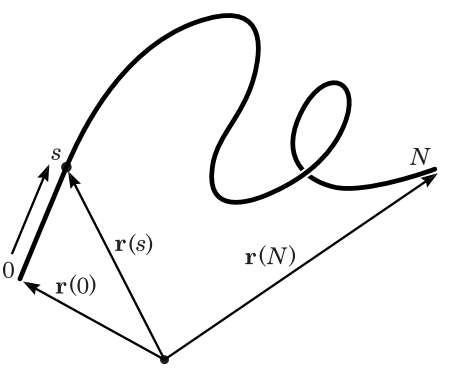
\includegraphics[scale=0.7]{./figures/1.png}
\caption{}
\end{figure}

图1:连续高斯链模型将聚合物的构型描述为空间曲线$\mathbf{r}(s)$,其中$s\in [0,N]$是路径参数。$\mathbf{r}(0)$和$\mathbf{r}(N)$是链端位置。

连续高斯链的势能可以写成
$$U_0[\mathbf{r}]=\frac{3k_BT}{2b^2}\int_{0}^{N} \mathrm{d}x\left| \frac{d\mathbf{r}(s)}{ds} \right|^2$$

其中$b$为链节的统计长度,$U_0[\mathbf{r}]$的方括号符号表示$U_0$是定义聚合物构型的空间曲线$\mathbf{r}(s)$的泛函。泛函是连续函数到数之间的映射。势能的形式与以下离散高斯链的方程密切相关
/home/gx/repository/文档例子
如果我们将$\frac{d\mathbf{r}(s)}{ds}$看作高分子长链上第$s$节(链节长度为$ds$)的拉伸形变,
然后,方程(2.42)对链的整个轮廓上每一个这样的微分段的谐波势贡献求和。
值得注意的是,在连续高斯链模型中,$s$并不表示弧长,而只是表示链上各段的参数指标。因此,拉伸$\frac{d\mathbf{r}(s)}{ds}$不是单位向量,而是大小可以自由波动。势能方程(2.42)通常称为“Edwards Hamiltonian”。

连续高斯链的配置构型配分函数可以写成
$$Z_0=\int \mathcal{D}\mathbf{r}~\exp(-\beta U_0[\mathbf{r}])$$

其中$\int \mathcal{D}\mathbf{r}$表示所有可能的描述聚合物的构型的空间曲线$\mathbf{r}(s)$上的泛函积分。这类泛函积分,又称路径积分,是量子力学和概率论领域(Feynman和Hibbs,1965)所熟悉的,其中$\mathbf{r}(s)$对应于量子粒子或布朗(Brownian)粒子在时间$s$的位置。实际上,方程(2.43)是经典扩散(布朗运动)路径积分描述中的维纳运动(Wiener motion)。

路径积分是一种复杂的数学对象,在定义和操作上需要一定的精确性(Simon,1979)。然而在这里,我们将非正式地和以物理的方式来对待这些对象。定义路径积分的一种方法是用$N_s+1$个等距轮廓点去离散离散路径,因此我们用$N_s+1$个点的空间位置逼近连续函数$\mathbf{r}(s)$,其中这$N_s+1$个点表示为向量$(\mathbf{r}_0,\mathbf{r}_1,...,\mathbf{r}_{N_s})$。这样,路径积分可以定义为$3(N_s+1)$维的普通积分
$$\int \mathcal{D}\mathbf{r}\approx \prod_{i=0}^{N_s} \int \, \mathrm{d} \mathbf{r}_i$$

其中,近似的质量随着$N_s$的增加而提高。当$N_s$有限时,连续高斯链的路径积分近似于有$N_s+1$个珠子的离散高斯链的配分函数。特别是,我们有一个近似
$$Z_0\approx \prod_{j=0}^{N_s} \int \, \mathrm{d} \mathbf{r}_j~\exp \left( -\frac{3}{2b^2\bigtriangleup s}\sum_{i=1}^{N_s}\left|\mathbf{r}_{i-1}-\mathbf{r}_i \right|^2 \right)$$

其中,其中一个$N_s$键的均方长度由$b^2\bigtriangleup s$给出,$\bigtriangleup s=N/N_s$是轮廓点之间的间距。

方程(2.45)的巧妙之处源于连续极限,因为$Z_0$尺度为$VN_s^{−(3/2)N_s}$,当$N_s\rightarrow \infty$时为零。通常我们对平均值感兴趣,它可以表示成两路径积分的比率。例如,连续高斯链的末端距向量的均方值可以表示为
$$R^2\equiv \left \langle \mathbf{R}\cdot \mathbf{R}\right \rangle _0=\frac{\int \mathcal{D}\mathbf{r}\left| \mathbf{r}(N)-\mathbf{r}(0) \right|^2~\exp(-\beta U_0[\mathbf{r}])}{\int \mathcal{D}\mathbf{r}~\exp(-\beta U_0[\mathbf{r}])}$$

其中分母只是配分函数$Z_0$。当根据方程(2.45)对分子和分母中的路径积分进行离散时,
发现奇异因子完全抵消,从而当$N_s\rightarrow \infty$时,$R^2$更好定义。此外,在路径积分的数值计算中,通常采用有限的$N_s$来避免奇异性。

定义路径积分的另一种方法是通过路径的谱表示。特别是,我们可以用扩充的一组完整的基函数$\lbrace \phi _0(s),\phi _1(s),... \rbrace$来表示空间曲线$\mathbf{r}(s)$
$$\mathbf{r}(s)=\sum_{p=0}^{\infty} \mathbf{a}_p \phi _P(s)$$

这是一种广义的傅里叶展开式,其展开式系数$\mathbf{a}_p$可以看作是广义傅里叶系数(见附录A)。对于在流体介质中自由悬浮的聚合物,基函数的一种方便的选择是符合“无拉伸”边界条件的余弦集$\frac{d\mathbf{r}(s)}{ds}\vert _{s=0}=\frac{d\mathbf{r}(s)}{ds}\vert _{s=N}=0$。这相当于余弦傅里叶级数表示
$$\mathbf{r}(s)=\mathbf{a}_0+2\sum_{p=1}^{\infty} \mathbf{a}_p \cos(p\pi s/N)$$
根据这些基函数的正交性可以求解傅里叶系数
$$\mathbf{a}_p=\frac{1}{N}\int_{0}^{N}  \mathrm{d}x~\cos(p\pi s/N)\mathbf{r}(s),p=0,1,2,...,\infty$$
这些模型在聚合物文献中被称为Rouse模型,在聚合物动力学理论中起着特别重要的作用(Doi和Edwards,1986)。实际上,$\mathbf{a}_0$可以解释为聚合物质心的位置,而$\mathbf{a}_p,p=1,2,3,...$,尺度越细则提供更多关于聚合物形状的信息。

利用Rouse谱表示,聚合物的所有构型(路径)上的积分可以解释为对所有Rouse模的积分的乘积。
$$\int \mathcal{D}\mathbf{r}= \prod_{p=0}^{\infty} \int \, \mathrm{d} \mathbf{a}_p$$
上述表达式右手边的对象是一个无穷维积分,所以我们再次遇到了分块函数$Z_0$的存在性问题。然而,这两个路径积分的比率证明是有限的,
为了数值计算的目的,我们取有限$P\gg1$使路径积分正则化(消除奇异点)
$$\int \mathcal{D}\mathbf{r}\approx \prod_{p=0}^{P} \int \, \mathrm{d} \mathbf{a}_p$$

为了说明Rouse模型在连续高斯链计算中的应用,用Rouse模型表示末端距向量的均方值是
$$\left | \mathbf{r}(N)-\mathbf{r}(0) \right |^2=16\sum_{p=1,3,...}^{\infty}\sum_{q=1,3,...}^{\infty} \mathbf{a}_p \cdot \mathbf{a}_q$$
这个数的平均值可以写为
$$\left \langle \left| \mathbf{R} \right|^2 \right \rangle _0=16\sum_{p=1,3,...}^{\infty}\sum_{q=1,3,...}^{\infty} \left \langle \mathbf{a}_p \cdot \mathbf{a}_q \right \rangle _0$$
其中,在Rouse模型中定义对象$f(\mathbf{a})$的平均值为
$$\left \langle f(\mathbf{a}) \right \rangle _0=\frac{\begin{matrix} \prod_{p=1}^{\infty} \int \, \mathrm{d} \mathbf{a}_p f(\mathbf{a})\exp(-\beta U_0(\mathbf{a})) \end{matrix}}{\begin{matrix} \prod_{p=1}^{\infty} \int \, \mathrm{d} \mathbf{a}_p \exp(-\beta U_0(\mathbf{a})) \end{matrix}}$$
在Rouse模型表达式中,方程(2.42)的势能是对角的
$$\beta U_0(\mathbf{a})=frac{1}{2}\sum_{p=1}^{\infty}\alpha (p)\mathbf{a}_p \cdot \mathbf{a}_p$$
其中$\alpha (p)=6\pi ^2p^2/(b^2N)$。注意,质心$p=0$模型是均匀分布。$p>0$模型都是统计独立的,是高斯分布,因此如下有(附录B)
$$\left \langle \mathbf{a}_p \cdot \mathbf{a}_q \right \rangle _0=\frac{3}{\alpha (p)}\delta _{pq}$$
替换到方程(2.53)将得
$$\left \langle \left| \mathbf{R} \right|^2 \right \rangle _0=\frac{8b^2N}{\pi ^2}\sum_{p=1,3,...}^{\infty}\frac{1}{p^2}=b^2N$$

由此我们得出结论:连续高斯链具有离散高斯链的性质,它的末端距向量的均方值由$R=bN^{1/2}$给出。类似用期望公式给出连续高斯链的旋转公式$R_g=b(N/6)^{1/2}$。


图2;用“随机过程”(stochastic process)方法从具有$s$段的连续高斯链的统计权重中构造出具有$s+\bigtriangleup s$段的连续高斯链末端位置的统计权重。



在探索连续高斯链模型的性质时,我们现在回到了随机过程方法。具体来说,考虑一个约化的分布函数$p_0 (\mathbf{r},s)$是很有用的,它描述了在$\mathbf {r}$处,一个连续的路径长度为$s$的高斯链。这个函数满足归一化条件的,即$\int \, \mathrm{d} \mathbf{r}~p_0(\mathbf{r},s)=1$。通过对离散高斯链的方程$p_0(\mathbf{r},j)=\int \, \mathrm{d} \mathbf{b}_j~\Phi(\mathbf{b}_j;\mathbf{r}-\mathbf{b}_j)p_0(\mathbf{r}-\mathbf{b}_j,j-1)$的类比,我们可以通过Chapman-Kolmogorov方程利用非常小的链的信息建立分布函数
$$p_0(\mathbf{r},s+\bigtriangleup s)=\int \, \mathrm{d}(\bigtriangleup \mathbf{r})\Phi(\bigtriangleup \mathbf{r};\mathbf{r}-\bigtriangleup \mathbf{r})p_0(\mathbf{r}-\bigtriangleup \mathbf{r},s)$$

\begin{figure}[H]
\centering
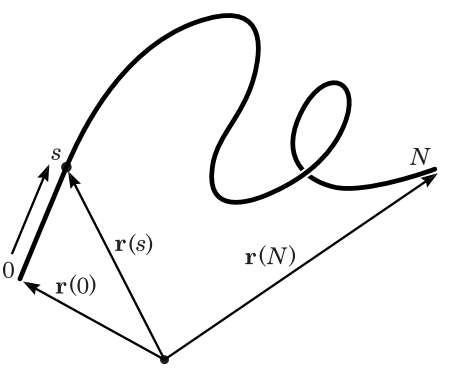
\includegraphics[scale=0.7]{./figures/1.png}
\caption{}
\end{figure}

图2说明了上述方程的物理内容,它依赖于连续链的最后一部分离散化。转移概率密度$\Phi(\bigtriangleup \mathbf{r};\mathbf{r}-\bigtriangleup \mathbf{r})$描述了路径长度$\bigtriangleup s$的链段的位移为$\bigtriangleup \mathbf{r}$的条件概率,从路径位置$s$处的$\mathbf{r}-\bigtriangleup \mathbf{r}$开始。连续高斯链的相关随机过程是稳定的,所以$\Phi =\Phi(\bigtriangleup \mathbf{r})$与起始位置和路径位置无关。$\Phi(\bigtriangleup \mathbf{r})$的表达式直接来自于连续高斯链方程(2.45)之前的离散化:
$$\Phi(\bigtriangleup \mathbf{r})=\left( \frac{3}{2\pi b^2 \bigtriangleup s} \right)^{3/2}\exp \left(- \frac{3\left| \bigtriangleup \mathbf{r} \right|^2}{2b^2 \bigtriangleup s} \right)$$

连续链模型的一个有用的特点是,Chapman-Kolmogorov积分方程可以归结为偏微分方程,在概率论中可归结为Fokker-Planck方程(van Kampenn,1981)和量子理论中的Feynman-Kac公式(Feynman和Hibbs,1965)。我们通过导出与方程(2.58)相结合的Fokker-Planck方程来说明这一点。这一推导是方程的两边通过泰勒展开。注意到在这种情况下,$\Phi(\bigtriangleup \mathbf{r};\mathbf{r}-\bigtriangleup \mathbf{r})$与初始位置$\mathbf{r}-\bigtriangleup \mathbf{r}$无关,我们不扩展转移概率。有
$$p_0(\mathbf{r},s)+\bigtriangleup s\frac{\partial}{\partial s}p_0(\mathbf{r},s)+O(\bigtriangleup s^2)=p_0(\mathbf{r},s)-\left \langle \bigtriangleup \mathbf{r} \right \rangle _\Phi \cdot \triangledown p_0 (\mathbf{r},s)+\frac{1}{2!}\left \langle \bigtriangleup \mathbf{r}  \bigtriangleup \mathbf{r} \right \rangle _\Phi:\triangledown \triangledown p_0(\mathbf{r},s)+O(\left \langle \bigtriangleup \mathbf{r}  \bigtriangleup \mathbf{r}  \bigtriangleup \mathbf{r} \right \rangle _\Phi)$$
其中,该方程中出现的$\Phi$平均定义为
$$\left \langle f(\bigtriangleup \mathbf{r}) \right \rangle _\Phi = \int \, \mathrm{d}(\bigtriangleup \mathbf{r})\Phi (\bigtriangleup \mathbf{r})f(\bigtriangleup \mathbf{r})$$
利用方程(2.59)的显式高斯形式,可以将方程(2.60)右侧的平均值计算为(附录B)
$$\left \langle \bigtriangleup \mathbf{r} \right \rangle _\Phi = 0$$
$$\left \langle \bigtriangleup \mathbf{r} \bigtriangleup \mathbf{r}_\beta \right \rangle _\Phi = \frac{b^2 \bigtriangleup s}{3}\delta_{\alpha \beta}$$
如果我们将这些式子带入方程(2.60)中,则$\bigtriangleup s \rightarrow \infty$时的分布函数$p_0(\mathbf{r},s)$满足Fokker-Planck方程
$$\frac{\partial}{\partial s}p_0(\mathbf{r},s)=\frac{b^2}{6}p_0(\mathbf{r},s)$$
因此,连续高斯链的Fokker-Planck方程给出的具有“扩散系数”$b^2/6$
的传统扩散方程的形式。该方程的解提供了关于端点段$p_0(\mathbf{r},s)$分布的完整信息。

Fokker-Planck方程是特别方便,因为有各种各样的分析和数值技术可用于求解偏微分方程。对于方程(2.64),对应于初始条件$p_0(\mathbf{r},s)=\delta(\mathbf{r})$的基本(格林函数)解是
$$p_0(\mathbf{r},s)=\left[ 3/(2 \pi sb^2) \right]^{3/2}\exp \left[ -3\left| \mathbf{r} \right|^2/(2sb^2) \right]$$

如果令$s=N,\mathbf{r}=\mathbf{R}$,则末端距矢量恢复成熟悉的高斯分布函数$p_0(\mathbf{R},N)=\left[ 3/(2 \pi N b^2) \right]^{3/2}\exp \left[ -3\left| \mathbf{R} \right|^2/(2N b^2) \right]$。在比单键大的尺度下,离散高斯链和连续高斯链明显具有相同的链端分布函数。使用连续链的优点是它允许用偏微分方程进行计算。这一优势将在第三章中变得更加明显,在第三章中,我们将考虑有外势的链。
\nocite{*}
%\bibliography{ref}
\end{document}